\documentclass[12pt, letterpaper]{article}
\usepackage[utf8]{inputenc}
%\usepackage[T1]{fontenc}
\usepackage[czech]{babel}
\usepackage{indentfirst}
\usepackage{tikz}
\usepackage{listings}
\usepackage{caption}
\usepackage{float}
\usepackage{qtree}
\usepackage{color,soul}
\PassOptionsToPackage{hyphens}{url}\usepackage{hyperref}
\usepackage{graphicx}
\usepackage[normalem]{ulem}
%%%
%%%
\begin{document}
%
\lstset{moredelim=[is][\sout]{@}{@}}
\lstset{escapeinside={(*}{*)}}
%%%
%%%
%%%
\section{Gramatika,  převod - NKA, DKA}
Gramatika zadání.
\begin{lstlisting}
S -> bA | bB | aS
A -> abA | bcB | e
B -> bA | cba
@C -> aS | ab | e@
\end{lstlisting}

Stav C je vyškrtnut, protože se do něj nelze dostat z žádného jiného stavu a není možné logicky odvodit, co stav reprezentuje a jak by se do něj mělo být možné dostat.

Zadaná gramatika převedena do regulárního tvaru.
\begin{lstlisting}
S -> bA | bB | aS
A -> aA(*$_1$*) | bB(*$_1$*) | e
A(*$_1$*) -> bA
B(*$_1$*) -> cB
B -> bA | cB(*$_2$*)
B(*$_2$*) -> bB(*$_3$*)
B(*$_3$*) -> aB(*$_4$*)
B(*$_4$*) -> e
\end{lstlisting}
%%%
%%%
\begin{figure}[H]
\begin{center}
\begin{tikzpicture}[scale=0.2]
\tikzstyle{every node}+=[inner sep=0pt]
\draw [black] (13.3,-21.7) circle (3);
\draw (13.3,-21.7) node {$S$};
\draw [black] (29.1,-13.4) circle (3);
\draw (29.1,-13.4) node {$A$};
\draw [black] (29.1,-13.4) circle (2.4);
\draw [black] (29.1,-30.6) circle (3);
\draw (29.1,-30.6) node {$B$};
\draw [black] (37.5,-36.6) circle (3);
\draw (37.5,-36.6) node {$exit$};
\draw [black] (15.96,-20.3) -- (26.44,-14.8);
\fill [black] (26.44,-14.8) -- (25.5,-14.72) -- (25.97,-15.61);
\draw (22.31,-18.05) node [below] {$b$};
\draw [black] (15.91,-23.17) -- (26.49,-29.13);
\fill [black] (26.49,-29.13) -- (26.03,-28.3) -- (25.54,-29.17);
\draw (20.09,-26.65) node [below] {$b$};
\draw [black] (10.958,-19.844) arc (259.34618:-28.65382:2.25);
\draw (9.36,-15.09) node [above] {$a$};
\fill [black] (13.35,-18.71) -- (13.99,-18.02) -- (13,-17.83);
\draw [black] (27.777,-10.72) arc (234:-54:2.25);
\draw (29.1,-6.15) node [above] {$ab$};
\fill [black] (30.42,-10.72) -- (31.3,-10.37) -- (30.49,-9.78);
\draw [black] (29.1,-16.4) -- (29.1,-27.6);
\fill [black] (29.1,-27.6) -- (29.6,-26.8) -- (28.6,-26.8);
\draw (28.6,-22) node [left] {$bc$};
\draw [black] (29.1,-27.6) -- (29.1,-16.4);
\fill [black] (29.1,-16.4) -- (28.6,-17.2) -- (29.6,-17.2);
\draw (29.6,-22) node [right] {$a$};
\draw [black] (31.54,-32.34) -- (35.06,-34.86);
\fill [black] (35.06,-34.86) -- (34.7,-33.98) -- (34.12,-34.8);
\draw (31.13,-34.1) node [below] {$cba$};
\end{tikzpicture}
\end{center}
\caption{Automat zadané gramatiky (nedeterministický)}
\label{automata_1}
\end{figure}

V obrázku \ref{automata_1} existuje stav pojmenován jako \texttt{exit}, který ale není v gramatice. Tento stav byl přidán, aby reprezentoval výstup ze stavu B sekvencí \textbf{cba}, protože použitý nástroj pro kreslení automatu neumožňuje volně mířící šipky.
%%%
\vspace{50px}
%%%
\begin{figure}[H]
\begin{center}
\begin{tikzpicture}[scale=0.2]
\tikzstyle{every node}+=[inner sep=0pt]
\draw [black] (9.2,-14.8) circle (3);
\draw (9.2,-14.8) node {$S$};
\draw [black] (23.1,-9.9) circle (3);
\draw (23.1,-9.9) node {$A$};
\draw [black] (23.1,-9.9) circle (2.4);
\draw [black] (23.1,-21.7) circle (3);
\draw (23.1,-21.7) node {$B$};
\draw [black] (38.3,-9.9) circle (3);
\draw (38.3,-9.9) node {$A_1$};
\draw [black] (38.3,-21.7) circle (3);
\draw (38.3,-21.7) node {$B_1$};
\draw [black] (23.1,-32) circle (3);
\draw (23.1,-32) node {$B_2$};
\draw [black] (32.3,-32) circle (3);
\draw (32.3,-32) node {$B_3$};
\draw [black] (42,-32) circle (3);
\draw (42,-32) node {$B_4$};
\draw [black] (42,-32) circle (2.4);
\draw [black] (6.469,-13.588) arc (273.80557:-14.19443:2.25);
\draw (3.81,-9.12) node [above] {$a$};
\fill [black] (8.5,-11.89) -- (8.95,-11.06) -- (7.95,-11.13);
\draw [black] (12.03,-13.8) -- (20.27,-10.9);
\fill [black] (20.27,-10.9) -- (19.35,-10.69) -- (19.68,-11.63);
\draw (17.17,-12.88) node [below] {$b$};
\draw [black] (11.89,-16.13) -- (20.41,-20.37);
\fill [black] (20.41,-20.37) -- (19.92,-19.56) -- (19.47,-20.46);
\draw (15.05,-18.76) node [below] {$b$};
\draw [black] (26.1,-9.9) -- (35.3,-9.9);
\fill [black] (35.3,-9.9) -- (34.5,-9.4) -- (34.5,-10.4);
\draw (30.7,-10.4) node [below] {$a$};
\draw [black] (25.47,-11.74) -- (35.93,-19.86);
\fill [black] (35.93,-19.86) -- (35.6,-18.97) -- (34.99,-19.76);
\draw (29.58,-16.3) node [below] {$b$};
\draw [black] (35.3,-9.9) -- (26.1,-9.9);
\fill [black] (26.1,-9.9) -- (26.9,-10.4) -- (26.9,-9.4);
\draw (30.7,-9.4) node [above] {$b$};
\draw [black] (35.3,-21.7) -- (26.1,-21.7);
\fill [black] (26.1,-21.7) -- (26.9,-22.2) -- (26.9,-21.2);
\draw (30.7,-21.2) node [above] {$c$};
\draw [black] (23.1,-18.7) -- (23.1,-12.9);
\fill [black] (23.1,-12.9) -- (22.6,-13.7) -- (23.6,-13.7);
\draw (23.6,-15.8) node [right] {$b$};
\draw [black] (23.1,-24.7) -- (23.1,-29);
\fill [black] (23.1,-29) -- (23.6,-28.2) -- (22.6,-28.2);
\draw (22.6,-26.85) node [left] {$c$};
\draw [black] (26.1,-32) -- (29.3,-32);
\fill [black] (29.3,-32) -- (28.5,-31.5) -- (28.5,-32.5);
\draw (27.7,-32.5) node [below] {$b$};
\draw [black] (35.3,-32) -- (39,-32);
\fill [black] (39,-32) -- (38.2,-31.5) -- (38.2,-32.5);
\draw (37.15,-32.5) node [below] {$a$};
\end{tikzpicture}
\end{center}
\caption{Automat regulární gramatiky (nedeterministický)}
\label{automata_2}
\end{figure}
%%%
\begin{table}[H]
\begin{center}
\begin{tabular}{| c || c | c | c |}
%% header
\hline
	\textbf{Stav} 			& \textbf{a} 	& \textbf{b} 	& \textbf{c}
%% body
\\\hline
	$\rightarrow$ S 		& S 		& \{A, B\} 	& $\emptyset$
\\\hline
	$\leftarrow$ \{A, B\} 		& $A_1$ 	& \{$B_1$, A\} 	& $B_2$
\\\hline
	$\leftarrow$ \{$B_1$, A\} 	& $A_1$ 	& \{$B_1$, A\} 	& \{A, B\}
\\\hline
	$A_1$				& $\emptyset$ 	& \{A, B\}	& $\emptyset$
\\\hline
	$B_2$				& $\emptyset$ 	& $B_3$		& $\emptyset$
\\\hline
	$B_3$				& $B_4$ 	& $\emptyset$	& $\emptyset$
\\\hline
	$\leftarrow$$B_4$		& $\emptyset$ 	& $\emptyset$	& $\emptyset$
\\\hline
\end{tabular}
\end{center}
\caption{Převedení gramatiky na deterministickou}
\label{table_1}
\end{table}
%

Stavy \{A, B\} a \{$B_1$, A\} budou dále označovány jako C a D (ve stejném pořadí) a nahrazují původní stavy A a B.
%%%

\begin{figure}[H]
\begin{center}
\begin{tikzpicture}[scale=0.2]
\tikzstyle{every node}+=[inner sep=0pt]
\draw [black] (9.2,-14.8) circle (3);
\draw (9.2,-14.8) node {$S$};
\draw [black] (23.1,-32) circle (3);
\draw (23.1,-32) node {$B_2$};
\draw [black] (32.3,-32) circle (3);
\draw (32.3,-32) node {$B_3$};
\draw [black] (42,-32) circle (3);
\draw (42,-32) node {$B_4$};
\draw [black] (42,-32) circle (2.4);
\draw [black] (23.1,-14.8) circle (3);
\draw (23.1,-14.8) node {$C$};
\draw [black] (23.1,-14.8) circle (2.4);
\draw [black] (36.7,-14.8) circle (3);
\draw (36.7,-14.8) node {$A1$};
\draw [black] (36.7,-23.4) circle (3);
\draw (36.7,-23.4) node {$D$};
\draw [black] (36.7,-23.4) circle (2.4);
\draw [black] (6.469,-13.588) arc (273.80557:-14.19443:2.25);
\draw (3.81,-9.12) node [above] {$a$};
\fill [black] (8.5,-11.89) -- (8.95,-11.06) -- (7.95,-11.13);
\draw [black] (26.1,-32) -- (29.3,-32);
\fill [black] (29.3,-32) -- (28.5,-31.5) -- (28.5,-32.5);
\draw (27.7,-32.5) node [below] {$b$};
\draw [black] (35.3,-32) -- (39,-32);
\fill [black] (39,-32) -- (38.2,-31.5) -- (38.2,-32.5);
\draw (37.15,-32.5) node [below] {$a$};
\draw [black] (12.2,-14.8) -- (20.1,-14.8);
\fill [black] (20.1,-14.8) -- (19.3,-14.3) -- (19.3,-15.3);
\draw (16.15,-15.3) node [below] {$b$};
\draw [black] (23.1,-17.8) -- (23.1,-29);
\fill [black] (23.1,-29) -- (23.6,-28.2) -- (22.6,-28.2);
\draw (22.6,-23.4) node [left] {$c$};
\draw [black] (36.7,-20.4) -- (36.7,-17.8);
\fill [black] (36.7,-17.8) -- (36.2,-18.6) -- (37.2,-18.6);
\draw (37.2,-19.1) node [right] {$a$};
\draw [black] (26.1,-14.8) -- (33.7,-14.8);
\fill [black] (33.7,-14.8) -- (32.9,-14.3) -- (32.9,-15.3);
\draw (29.9,-15.3) node [below] {$a$};
\draw [black] (25.64,-16.4) -- (34.16,-21.8);
\fill [black] (34.16,-21.8) -- (33.76,-20.95) -- (33.22,-21.79);
\draw (28.79,-19.6) node [below] {$b$};
\draw [black] (34.16,-21.8) -- (25.64,-16.4);
\fill [black] (25.64,-16.4) -- (26.04,-17.25) -- (26.58,-16.41);
\draw (30.89,-18.6) node [above] {$c$};
\draw [black] (33.7,-14.8) -- (26.1,-14.8);
\fill [black] (26.1,-14.8) -- (26.9,-15.3) -- (26.9,-14.3);
\draw (29.9,-14.3) node [above] {$b$};
\draw [black] (39.38,-22.077) arc (144:-144:2.25);
\draw (43.95,-23.4) node [right] {$b$};
\fill [black] (39.38,-24.72) -- (39.73,-25.6) -- (40.32,-24.79);
\end{tikzpicture}
\end{center}
\caption{Automat podle tabulky (deterministický)}
\label{automata_3}
\end{figure}
%%%
%%%
%%%
\newpage
\section{Automat dělitelnosti 5ti binárního čísla}
Přesně takovýto automat a jeho princip je výborně popsán zde \url{https://math.stackexchange.com/questions/4027896/pattern-for-all-the-binary-chains-divisible-by-5}. Tento zdroj byl použit.
%
\begin{figure}[H]
\begin{center}
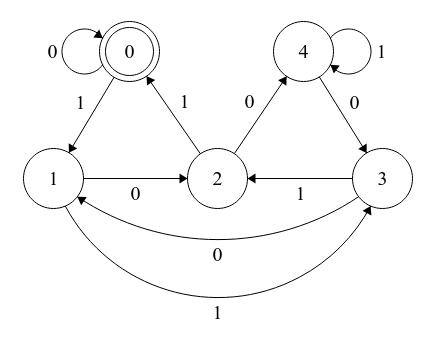
\includegraphics[width=0.75\textwidth]{division5.png}
\caption{Automat dělitenosti 5ti binárního čísla}
\label{automata_division_5}
\end{center}
\end{figure}
%
\begin{table}[H]
\begin{center}
\begin{tabular}{| c | c || c | c |}
%% header
\hline
	\textbf{k}	& \textbf{b}	& \textbf{2k + b}	& \textbf{(2k + b) mod 5}
%% body
\\\hline
	0		& 0 		& 0 			& 0
\\\hline
	0		& 1 		& 1 			& 1
\\\hline
	1		& 0 		& 2 			& 2
\\\hline
	1		& 1 		& 3 			& 3
\\\hline
	2		& 0 		& 4 			& 4
\\\hline
	2		& 1 		& 5 			& \textbf{0} (mod 5)
\\\hline
	3		& 0 		& 6 			& 1
\\\hline
	3		& 1 		& 7 			& 2
\\\hline
	4		& 0 		& 8 			& 3
\\\hline
	4		& 1 		& 9 			& 4

\\\hline
\end{tabular}
\end{center}
\caption{Funkčnost automatu dělitolnosti 5ti binárního čísla}
\label{table_division_5}
\end{table}
%

Tabulka \ref{table_division_5} popisuje průchod automatem a způsob principu automatu. Začínáme ve stavu 0 (\textbf{k} - zbytek po dělení 5ti) a poté přijímáme binární číslo \textbf{b}. Nyní provedeme \textbf{2k + b}, kde \textbf{k} je číslo stavu a \textbf{b} je načtená binární hodnota. Načtením hodnoty \textbf{b} se mění vstupní číslo a je třeba přepnout automat do správného stavu. Ten je získán provedením operace \textbf{2k + b mod 5}, protože hledáme číslo dělitelné 5ti a proto jsou stavy automatu zbytky po dělení 5ti (mod 5).
%%%
%%%
%%%
\newpage
\section{Sestavení gramatiky popisující jazyk reg. výrazů}
% TODO : tuto rve, nevim proc
\subsubsection{Vysvětlivky}
\begin{lstlisting}
a ... ASCII znak
b ... +| ... nebo
* ... iterace
() ... priorita
\end{lstlisting}
%
\subsubsection{Gramatika}
\begin{lstlisting}
S -> aA | (aAB
(*$S_1$*) -> aA | (aAB | (**$S_1$*) | e
A -> a(*$S_1$*) | ba(*$S_1$*) | (*$S_1$*) | e
B -> )(*$S_1$*) | )e
\end{lstlisting}
%
%regex1: a(b|c)*
\subsection{Příklad 1: a(b$|$c)*}
Pozor: v příkladu jsou \textbf{a,b,c} ASCII znaky, ale v grafu \textbf{a} reprezentuje ASCII všechny znaky a \textbf{b} reprezentuje \textbf{nebo}.

S $\rightarrow$ \hl{aA} $\rightarrow$ a\hl{$S_1$} $\rightarrow$ a\hl{(aAB} 
$\rightarrow$ a(a\hl{ba$S_1$}B $\rightarrow$ a(abaB $\rightarrow$ a(aba\hl{)$S_1$} $\rightarrow$
a(aba)\hl{*$S_1$} $\rightarrow$ a(aba)*
\newline
\newline
\newline
\Tree	[.S 	[.A \textit{a}
			[.$S_1$ \textit{(a}
				[.A \textit{ba}
					[.$S_1$ \textit{e}
					]
				]
				[.B \textit{)}
					[.$S_1$ \textit{*}
						[.$S_1$ \textit{e}
						]
					]
				]
			]
		]
	]
%regex2: (a(bc))
\subsection{Příklad 2: (a(bc))}
Pozor: v příkladu jsou \textbf{a,b,c} ASCII znaky, ale v grafu \textbf{a} reprezentuje ASCII všechny tyto znaky.

S $\rightarrow$ \hl{(aAB} $\rightarrow$ (a\hl{$S_1$}B
$\rightarrow$ (a\hl{(aAB}B $\rightarrow$ 
(a(a\hl{a$S_1$}BB $\rightarrow$ (a(aaBB
$\rightarrow$ (a(aa\hl{)}B $\rightarrow$ 
(a(aa)\hl{)} $\rightarrow$ (a(aa))
\newline
\newline
\newline
\Tree	[.S 	[.A \textit{(a}
			[.$S_1$ \textit{(a}
				[.A \textit{a}
					[.$S_1$ \textit{e}
					]
				]
				[.B \textit{)e}
				]
			]
		]
		[.B \textit{)e}
		]
	]
%%%
%%%
\end{document}
